% Overleaf: upload this whole slides/ folder (main.tex + figures/) and compile with pdfLaTeX.
\documentclass[aspectratio=169,11pt]{beamer}
\usetheme[progressbar=frametitle]{metropolis}
\usepackage{booktabs}
\usepackage{tikz}
\usetikzlibrary{arrows.meta,positioning}
\graphicspath{{figures/}}

\definecolor{qblue}{HTML}{2A78D6}
\definecolor{qorange}{HTML}{EB6834}
\definecolor{qgreen}{HTML}{1BAF7A}
\setbeamercolor{alerted text}{fg=qorange}

\title{Can Grover's Algorithm Solve Real Puzzles on Noisy Quantum Computers?}
\subtitle{Grover search for SAT, graph colouring and Sudoku, compared with classical search under noise}
\author{Your Name}
\institute{Supervisor: Prof.\ Name}
\date{\today}

\begin{document}

\maketitle

%------------------------------------------------------------------------------
\begin{frame}{The question in one line}
\begin{center}
\Large Grover's algorithm is famous for being faster at search.\\[0.4em]
\textbf{Is it still faster on real puzzles, once the quantum computer makes mistakes?}
\end{center}
\vspace{1em}
\begin{itemize}
\item I built Grover search for \textbf{three kinds of puzzles}: 3-SAT, graph colouring and $4\times4$ Sudoku.
\item I compared it with \textbf{normal (classical) ways} of solving them.
\item I added \textbf{realistic noise} and found the point where Grover stops winning.
\end{itemize}
\end{frame}

%------------------------------------------------------------------------------
\begin{frame}{Grover's algorithm in one slide}
\begin{columns}[T]
\column{0.55\textwidth}
\begin{itemize}
\item You have $N$ possible answers; $M$ of them are correct.
\item Checking one by one takes about $N/M$ tries.
\item Grover needs only about $\sqrt{N/M}$ tries.
\item This is the famous \textbf{quadratic speedup}.
\end{itemize}
\column{0.42\textwidth}
\begin{tabular}{@{}rrr@{}}
\toprule
$N$ & checking & Grover \\
\midrule
16 & $\approx$ 8 & 3 \\
1{,}000 & $\approx$ 500 & 25 \\
1{,}000{,}000 & $\approx$ 500{,}000 & 785 \\
\bottomrule
\end{tabular}\\[0.4em]
{\small (one correct answer)}
\end{columns}
\vspace{1em}
\alert{The catch:} Grover needs an \textbf{oracle}, a circuit that recognises a correct answer.
\end{frame}

%------------------------------------------------------------------------------
\begin{frame}{What makes this project different}
\begin{columns}[T]
\column{0.48\textwidth}
\textbf{Most online demos}
\begin{itemize}
\item The oracle is told ``the answer is \texttt{101}''.
\item If you already know the answer, there is nothing to search for.
\item It's a demo, not a real search.
\end{itemize}
\column{0.48\textwidth}
\textbf{This project}
\begin{itemize}
\item The oracle \textbf{only knows the rules} of the puzzle.
\item It checks \emph{all} possible answers at once (superposition).
\item It \textbf{never sees the solution}, which is how a real search would work.
\end{itemize}
\end{columns}
\end{frame}

%------------------------------------------------------------------------------
\begin{frame}{The three puzzles}
\begin{columns}[T]
\column{0.32\textwidth}
\textbf{3-SAT}\\[0.3em]
A logic formula:\\
{\small $(x_1 \lor \lnot x_2 \lor x_3)\land\dots$}\\[0.3em]
Find true/false values that make every bracket true.
\column{0.32\textwidth}
\textbf{Graph colouring}\\[0.3em]
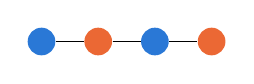
\begin{tikzpicture}[scale=0.8]
\foreach \i/\c in {0/qblue,1/qorange,2/qblue,3/qorange}
  \node[circle,fill=\c,minimum size=10pt,inner sep=0] (v\i) at (\i*0.9,0) {};
\draw (v0)--(v1)--(v2)--(v3);
\end{tikzpicture}\\[0.3em]
Colour the dots so that no two connected dots share a colour.
\column{0.32\textwidth}
\textbf{$4\times4$ Sudoku}\\[0.3em]
A mini Sudoku with 2--4 blanks.\\[0.3em]
Fill the blanks so that every row, column and box has 1--4 once.
\end{columns}
\vspace{1.2em}
All three are \textbf{constraint satisfaction problems}: a list of rules, and you want an answer that obeys all of them.
\end{frame}

%------------------------------------------------------------------------------
\begin{frame}{How the oracle works}
\begin{center}
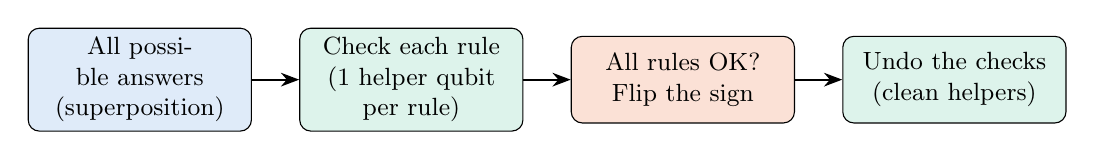
\begin{tikzpicture}[node distance=0.6cm, box/.style={draw, rounded corners, align=center, minimum height=1.1cm, text width=2.6cm, font=\small}, >=Stealth]
\node[box, fill=qblue!15] (a) {All possible answers\\(superposition)};
\node[box, fill=qgreen!15, right=of a] (b) {Check each rule\\(1 helper qubit\\per rule)};
\node[box, fill=qorange!20, right=of b] (c) {All rules OK?\\Flip the sign};
\node[box, fill=qgreen!15, right=of c] (d) {Undo the checks\\(clean helpers)};
\draw[->, thick] (a)--(b); \draw[->, thick] (b)--(c); \draw[->, thick] (c)--(d);
\end{tikzpicture}
\end{center}
\vspace{0.6em}
Every puzzle is built from just \textbf{3 building blocks}:
\begin{itemize}
\item \texttt{Clause}: ``at least one of these is true'' (SAT)
\item \texttt{NotEqual}: ``these two must be different'' (colouring, Sudoku)
\item \texttt{InSet}: ``this cell must be one of these values'' (Sudoku)
\end{itemize}
\textbf{Correctness:} the tests run every possible input through every oracle and check that it marks exactly the real solutions. All tests pass.
\end{frame}

%------------------------------------------------------------------------------
\begin{frame}{How I compared fairly}
Every method is scored in the same unit: \textbf{how many answers it has to check}.
\vspace{0.5em}
\begin{itemize}
\item \textbf{Brute force:} try answers in random order.
\item \textbf{DPLL:} the classic ``smart'' SAT solver that reasons about the rules.
\item \textbf{WalkSAT:} random local search.
\item \textbf{Grover:} run the circuit, measure, check the answer on a normal computer, and repeat if it's wrong:
\[
\text{Grover cost} = \frac{\text{iterations}+1}{\text{chance of success}}
\]
\end{itemize}
Noise lowers the chance of success, so Grover has to repeat more often.
\end{frame}

%------------------------------------------------------------------------------
\begin{frame}{Adding noise}
\begin{itemize}
\item Quantum gates sometimes go wrong. The most error-prone ones are the \textbf{two-qubit gates (CNOTs)}.
\item $p_2$ = the chance that one CNOT goes wrong.\\
\quad $p_2 = 10^{-3}$ means about \textbf{1 in 1000 CNOTs fails}.
\item Today's IBM hardware: roughly $10^{-3}$ to $10^{-2}$.
\end{itemize}
\vspace{0.6em}
\begin{block}{Key number: the threshold $p_2^*$}
The noise level where Grover becomes \textbf{worse than brute force}.\\
Above $p_2^*$, the quantum computer is no longer worth using for this problem.
\end{block}
\end{frame}

%------------------------------------------------------------------------------
\begin{frame}{Result 1: noise kills the advantage quickly}
\centering
\includegraphics[width=\textwidth,height=0.8\textheight,keepaspectratio]{csp_noise_heatmap.png}\\
{\small Each cell = chance of getting a correct answer. Outlined = Grover still beats brute force.}
\end{frame}

%------------------------------------------------------------------------------
\begin{frame}{Result 1: in numbers}
\begin{columns}[T]
\column{0.5\textwidth}
\begin{tabular}{@{}lrr@{}}
\toprule
Puzzle & CNOTs & $p_2^*$ \\
\midrule
Colouring, 4 dots & 80 & $1.0\times10^{-2}$ \\
Colouring, 6 dots & 352 & $4.8\times10^{-3}$ \\
Sudoku, 2 blanks & 204 & $4.2\times10^{-3}$ \\
Sudoku, 4 blanks & 1488 & $1.8\times10^{-3}$ \\
3-SAT, 3 variables & 522 & $7.4\times10^{-4}$ \\
3-SAT, 4 variables & 932 & $8.5\times10^{-4}$ \\
\bottomrule
\end{tabular}
\column{0.46\textwidth}
\begin{itemize}
\item The advantage disappears at about \textbf{0.07\% to 1\%} error.
\item That is \alert{right where today's hardware is}.
\item \textbf{Bigger circuits break sooner}: more CNOTs, more chances for a mistake.
\item \textbf{SAT breaks first}, even though its circuits aren't the biggest. Why?
\end{itemize}
\end{columns}
\end{frame}

%------------------------------------------------------------------------------
\begin{frame}{Why SAT breaks first}
Grover only wins if its success chance stays above a \textbf{required level}:
\[
P_\text{req} = \frac{(\text{iterations}+1)(M+1)}{N+1}
\]
\begin{columns}[T]
\column{0.48\textwidth}
\textbf{3-SAT, 3 variables}
\begin{itemize}
\item Only $N=8$ possible answers.
\item Brute force needs only 4.5 checks.
\item Grover must succeed \alert{67\%} of the time to win.
\end{itemize}
\column{0.48\textwidth}
\textbf{Colouring, 6 dots}
\begin{itemize}
\item $N=64$ possible answers.
\item Brute force needs about 22 checks.
\item Grover only needs \textbf{23\%} success to win.
\end{itemize}
\end{columns}
\vspace{0.6em}
Small puzzles leave Grover \textbf{very little room for mistakes}.
\end{frame}

%------------------------------------------------------------------------------
\begin{frame}{Result 2: one simple formula predicts the threshold}
\begin{columns}[c]
\column{0.54\textwidth}
\small
Each CNOT error eats away a little success, so:
\[
p_2^* = \frac{\ln(P_\text{ideal}/P_\text{req})}{\alpha \cdot \text{(number of CNOTs)}}
\]
\begin{itemize}
\item Only \textbf{one constant} to fit: $\alpha \approx 0.78$.
\item Predicts every measured threshold within \textbf{about $\pm$12\%}.
\item Sudoku is held back to \textbf{test} the formula on unseen data.
\end{itemize}
{\footnotesize\textit{Preliminary: colouring and SAT done, Sudoku still running.}}
\column{0.42\textwidth}
\includegraphics[width=\textwidth,height=0.75\textheight,keepaspectratio]{study_decay_model.png}
\end{columns}
\end{frame}

%------------------------------------------------------------------------------
\begin{frame}{What the formula says about big problems}
\begin{itemize}
\item Bigger puzzle $\Rightarrow$ Grover needs more iterations $\Rightarrow$ \textbf{many more CNOTs} (grows like $\sqrt{N}$).
\item The top of the formula grows only very slowly (like $\log N$).
\item So the threshold \textbf{keeps falling} as puzzles get bigger.
\end{itemize}
\vspace{0.5em}
\begin{block}{Example: 3-SAT with 20 variables (about a million possible answers)}
Needed error rate: about $\mathbf{10^{-5}}$, which is \alert{100 times better than today's best hardware}.
\end{block}
\vspace{0.3em}
Conclusion: useful Grover search on puzzles like these needs \textbf{error-corrected} quantum computers.
\end{frame}

%------------------------------------------------------------------------------
\begin{frame}{Result 3: building a cheaper oracle}
Two circuit tricks:
\begin{itemize}
\item \textbf{Relative-phase Toffolis:} cheaper gates that add small extra phases. Those phases cancel exactly when the oracle cleans up, and the tests confirm it.
\item \textbf{Reusing idle qubits} as helpers for the big multi-control gates.
\end{itemize}
\vspace{0.4em}
\begin{columns}[T]
\column{0.48\textwidth}
\textbf{On 3-SAT (4 variables)}
\begin{itemize}
\item CNOTs: 932 $\rightarrow$ \textbf{558} (40\% fewer)
\item Threshold: \textbf{$\times$1.75 higher}
\end{itemize}
\column{0.48\textwidth}
\textbf{But}
\begin{itemize}
\item On colouring the saving is small (2--12\%).
\item It is a constant-factor improvement, not a change in how the threshold scales.
\end{itemize}
\end{columns}
{\small\textit{Preliminary numbers; final run in progress.}}
\end{frame}

%------------------------------------------------------------------------------
\begin{frame}{Result 4: more solutions help Grover}
\begin{columns}[c]
\column{0.5\textwidth}
\includegraphics[width=\textwidth]{csp_success_vs_iterations.png}
\column{0.47\textwidth}
\begin{itemize}
\item More correct answers $\Rightarrow$ fewer iterations $\Rightarrow$ shorter circuit $\Rightarrow$ \textbf{less damage from noise}.
\item 1 solution: success drops 96\% $\rightarrow$ 49\% with noise.
\item 4 solutions: only 100\% $\rightarrow$ 88\%.
\item Don't know how many solutions there are? The \textbf{BBHT} version of Grover handles that at only \textbf{1.2--1.7$\times$} the cost.
\end{itemize}
\end{columns}
\end{frame}

%------------------------------------------------------------------------------
\begin{frame}{Result 5: the honest comparison with classical solvers}
\begin{columns}[c]
\column{0.55\textwidth}
\includegraphics[width=\textwidth]{csp_queries_vs_solutions_n4.png}
\column{0.42\textwidth}
\begin{itemize}
\item \textbf{Perfect} Grover uses the fewest checks.
\item With noise at $10^{-3}$, Grover is only about as good as \textbf{WalkSAT}.
\item On a 1-solution formula: noisy Grover needs \textbf{8.2} checks, the smart DPLL solver \textbf{4.7} steps.
\item Beating brute force $\neq$ beating the best classical method.
\end{itemize}
\end{columns}
\end{frame}

%------------------------------------------------------------------------------
\begin{frame}{Can error mitigation save it? (ZNE)}
\textbf{Zero-noise extrapolation (ZNE):} run the circuit with \emph{extra} noise, then extrapolate back to zero noise.
\vspace{0.5em}
\begin{itemize}
\item It \textbf{does} give a good \emph{estimate} of the success probability.
\item But search needs an \textbf{actual correct answer} from a measurement, not an estimate.
\item Every single shot still comes from the noisy circuit, and the extra-noise runs are even worse.
\end{itemize}
\vspace{0.5em}
\begin{block}{Analogy}
Knowing the class average on an exam doesn't give you the right answer sheet.
\end{block}
So ZNE doesn't help search. Methods that change the samples themselves (error \emph{detection}) are needed instead.
\end{frame}

%------------------------------------------------------------------------------
\begin{frame}{Real chip models}
\begin{itemize}
\item I also simulated copies of real IBM chips (\textbf{Brisbane, Torino, Kingston}) with their real calibration data.
\item Real chips don't connect every qubit to every other qubit, so extra swap gates are needed.
\item This \textbf{roughly doubles} the number of CNOTs, which makes things worse than the simple model.
\item The script to run on real IBM hardware (\texttt{hardware.py}) is ready.
\end{itemize}
\vspace{0.5em}
{\small\textit{Full device results are still running.}}
\end{frame}

%------------------------------------------------------------------------------
\begin{frame}{Limitations}
\begin{itemize}
\item \textbf{Small puzzles} (at most 13 qubits). Simulating noise gets extremely slow beyond about 15 qubits.
\item The simple noise model assumes every qubit can talk to every other one. The chip models fix this.
\item The chip models are snapshots: no crosstalk or drift.
\item Claims about big problems come from the formula, not from big simulations.
\item DPLL ``steps'' are not exactly the same unit as Grover checks, so that comparison shows a trend.
\end{itemize}
\end{frame}

%------------------------------------------------------------------------------
\begin{frame}{Where the project stands}
\begin{columns}[T]
\column{0.48\textwidth}
\textbf{Done}
\begin{itemize}
\item Oracles for 3 puzzle types, fully tested
\item Classical solvers + fair cost model
\item Noise study + figures
\item Interactive web app (Streamlit)
\item IEEE-format paper draft
\end{itemize}
\column{0.48\textwidth}
\textbf{In progress}
\begin{itemize}
\item Final large run: Sudoku instances, real-chip models, ZNE
\item Then: finish paper results and submit
\end{itemize}
\vspace{0.5em}
\textbf{Optional}
\begin{itemize}
\item Run on real IBM quantum hardware
\end{itemize}
\end{columns}
\end{frame}

%------------------------------------------------------------------------------
\begin{frame}{Take-home messages}
\begin{enumerate}
\item I built Grover oracles that \textbf{check rules}, not ones that already know the answer.
\item Grover's advantage disappears at \textbf{0.07\%--1\% gate error}, which is about today's hardware level.
\item A \textbf{one-constant formula} predicts when the advantage disappears, and it says bigger problems need much better hardware ($\sim10^{-5}$).
\item Smarter circuits help by a \textbf{constant factor}; ZNE does \textbf{not} help search.
\item Good classical solvers are \textbf{very hard to beat} at this scale.
\end{enumerate}
\vspace{1em}
\begin{center}
\Large Thank you! Questions?
\end{center}
\end{frame}

\end{document}
